\documentclass[a4paper,11pt]{ltjsarticle}
\usepackage{amsmath, mathtools, amssymb, fancyhdr, anyfontsize, subcaption, graphicx, url, enumitem, ascmac, tikz}
\usetikzlibrary{arrows}

\title{レポートの書き方とデータの統計処理}
\author{Y-teraya}
\date{}

\begin{document}

\pagestyle{fancy}
\lhead{レポートの書き方}
\rhead{\textbf{\thepage}\ }
\cfoot{}
\renewcommand{\footrulewidth}{0.4pt}

\maketitle
\definecolor{qqffff}{rgb}{0,1,1}

\section{はじめに}

本資料では,レポートの書き方,実験で得たデータの統計処理について取り扱う.
またデータは,実験で測定した\textbf{実測値},計算して求めた\textbf{理論値}の2つに分かれる.
任意のデータが\textbf{測定の不確かさの範囲}に含まれているのか検証し,実験精度を考察できるようにすることを目的とする.

\section{レポートの書き方}

\subsection{前提}

レポートは,以下の通りに書くことが基本である.

\begin{itemize}
    \item A4のレポート用紙を用いる.
    \begin{itemize}
        \item 罫線が書かれている側に文字を書き,裏には何も書かない.
    \end{itemize}
    \item ボールペン書きでかつ修正機の使用不可.
    \item 必ず表紙を付け,左上にホッチキス止め.
    \item 漢字ミス,送り仮名ミス,漢字で書くべきところが平仮名のようなことが無いようにする.
    \item グラフを綺麗に描く.
    \begin{itemize}
        \item 曲線のグラフに直線が含まれていない.
        \item 直線を定規で描く.\hfill など
    \end{itemize}
\end{itemize}

\subsection{「表紙」の書き方}

以下のことは,必ず記載すること.

\begin{itemize}
    \item 実験タイトル
    \item 実験者(共同実験者がいれば,記載のこと.)
    \item 実験日(可能であれば,温度と湿度も記載のこと.)
    \item 提出日
\end{itemize}

\clearpage

\subsection{「実験の目的」の書き方}

実験手順書を基に,簡潔に文章表現を変えて記述する.

\subsection{「実験の理論」の書き方}

実験の測定原理や利用する公式の記述をする.そして,式だけで1行とり番号を付け,すべての変数の定義をする.

例)電圧を$V\ [\mathrm{V}]$,抵抗を$R\ [\mathrm{\Omega}]$,電流を$I\ [\mathrm{mA}]$ とすると,

\begin{equation}
    V = RI
\end{equation}

\begin{itemize}
    \item 電圧を$V\ [\mathrm{V}]$ のように,変数の定義をする.
    \item $V = RI$という式に,(1)という番号を付ける.
    \item なぜこの式になるのか簡単に論じる.
\end{itemize}

\subsection{「実験方法」の書き方}

実験で用いた器具や試薬類を書き出す.また,実験の方法を,\textbf{実際に行った順番で}簡潔に書き並べる.

注)実験と関係のない内容(「スイッチを入れる」など)の記述は避け,本質的な手順とその目的のみを記述すること.

\subsection{「実験結果」の書き方}

\begin{itemize}
  \item 実験結果をや測定した実測値を記述する.また,得られた結果を図表やグラフを用いて\textbf{見やすく分かりやすい}表現にする.
  \item 図表を用いる場合,「 \bigcirc\bigcirc の結果,表1のような結果が得られた.」のようにそれらの説明を文章中に明記する.
  \item また,図・グラフは「図1」,表は「表1」のように通し番号をつけ,タイトルをつける.
  \item 実験理論の数式を利用した場合は,必ず式番号を示す.
\end{itemize}

\section{「考察」の書き方}

あくまでも考察は,\textbf{自身で考えたこと}を記す.課題や\textbf{感想}や\textbf{結果}ではない.

\vspace{10pt}

(感想)\ 本実験系は,\bigcirc\bigcirc で\textbf{大変だった}.

(結果)\ 実測値から計算された\textbf{結果}は,\bigcirc\bigcirc だった.


\clearpage

例えば,測定により得られた結果から誤差などの原因や改善点を挙げる.また,実測値と理論値の比較や失敗した場合はその要因を書くと良いだろう.

\section{「参考文献」の書き方}

引用・参考にした文献を以下のように記述する.また,カンマ・ピリオドの後には必ず,半角スペースを入れる.

\begin{enumerate}[label={[}\arabic*{]}]
  \item 鈴木花子:\bigcirc\bigcirc の測定,\square\square 出版,1981.
  \item 山田太郎:\bigcirc\bigcirc 方法の評価,\square\square 雑誌,Vol. 3,No. 1,pp. 25-60,2002.
\end{enumerate}

基本的には,

\begin{enumerate}[label={[}\arabic*{]}]
  \item 【著者名】:【タイトル】,【出版社】,【ページ数】,【発行年日】.
  \item 【著者名】;【タイトル】,【URL】,【閲覧年日】.
\end{enumerate}


で記述する.また,どの文章で参考にしたのかを明示するために,文章の最後に上付きで番号を付ける.

例)〜〜〜〜〜〜〜〜〜〜〜${}^{[1]}$.

\section{表の書き方}

表の書き方を以下に示す.表1の間違いは以下に記載している.このような書き方をしないようにすること.

\begin{table}[htbp]
  \begin{minipage}[b]{0.49\linewidth}
    \centering
    \begin{tabular}{|c|c|c|c|c|l|}
        \hline
        電圧 {\color{magenta}$^③$} & 0 & 0.20 & 0.40 & 0.60 & $\cdots$\\
        \hline
        電流 {\color{magenta}$^③$} &   &      &      &      & {\color{magenta}$^②$} \\
        \hline
    \end{tabular}
    \caption{ダメな表の例 {\color{magenta}$^①$}}
  \end{minipage}
  \begin{minipage}[b]{0.49\linewidth}
    \centering
    \caption{正しい表の例}
    \begin{tabular}{cccccc}
        \hline
        電圧 [V] & 0 & 0.20 & 0.40 & 0.60 & $\cdots$ \\
        電流 [mA] &  &      &      &      &      \\
        \hline
    \end{tabular}
  \end{minipage}
\end{table}

\begin{enumerate}[label={\color{magenta}\arabic*. }]
    \item 表題は\textbf{上に書く}.
    \item 表の\textbf{縦線は不要}.
    \item 単位を明記すること.
    \item 有効数字を合わせること.
    \item \textbf{表の後にグラフが来る}.( \because\ 表を基にしてグラフ化する.)
    \item 実測値を統計処理した場合は\textbf{有効数字}で書き,理論値や文献値と比較する.
\end{enumerate}

\clearpage

\section{グラフの書き方}

グラフの書き方を以下に示す.図1の間違いは以下に記載している.このような書き方をしないようにすること.当たり前ではあるが,グラフは\textbf{方眼範囲の中央}に描く.

\begin{figure}[h]
    \centering
    \begin{minipage}[b]{0.49\columnwidth}
        \centering
        \begin{tikzpicture}[line cap=round,line join=round,>=triangle 45,x=1cm,y=1cm,scale=0.28]

            % 方眼範囲
            \draw [color=qqffff,fill=qqffff,fill opacity=0.08] (-2,22) -- (-2,-3.5) -- (16,-3.5) -- (16,22) -- cycle;

            % プロット範囲
            \draw [fill=black,fill opacity=0.08] (0,20) -- (0,-3.5) -- (14,-3.5) -- (14,20) -- cycle;

            % 全体範囲
            \draw (-4.5,25) -- (-4.5,-6.5) -- (18.5,-6.5) -- (18.5,25) -- cycle;

            % グラフ軸
            \draw [line width=2pt,<-] (14,-3.5) -- (0,-3.5);
            \draw [line width=2pt,<-] (0,20) -- (0,-3.5);
            \draw (0,-3.5) node[below left] {{\color{magenta}$^⑦$}O};
            \draw (14,-3.5) node[below] {\color{magenta}$^④$};
            \draw (0,20) node[left] {\color{magenta}$^④$};

            % グラフ
            \draw [line width=1.5pt,cyan] (0,-1) -- (8,5) --(8.5,3) -- (14,8);
            \draw [line width=1.5pt,dashed,orange] (0,0) -- (14,15);

            % 点〇
            \draw [fill=cyan,draw=cyan] (3,1) circle (3pt);
            \draw [line width=1.5pt,cyan] (3,1) circle (13pt);
            \draw [fill=cyan,draw=cyan] (8.5,3) circle (3pt);
            \draw [line width=1.5pt,cyan] (8.5,3) circle (13pt);
            \draw [fill=cyan,draw=cyan] (14,7.5) circle (3pt);
            \draw [line width=1.5pt,cyan] (14,7.5) circle (13pt);
            \draw (14,7.5) node[above left] {\color{magenta}$^⑤$};

            % 点◇
            \draw [fill=orange,draw=orange] (4,5) circle (3pt);
            \draw (4,5) node[above left] {\color{magenta}$^⑥$};
            \draw (8.5,3) node[below left] {\color{magenta}$^⑩$};
            \draw [fill=orange,draw=orange] (9,9) circle (3pt);
            \draw [fill=orange,draw=orange] (12,13) circle (3pt);

            % 軸の名前
            \draw (7,-3.5) node[below] {{\color{magenta}$^③$}\textbf{電圧} [V]};
            \draw (7,20) node[above] {図1 抵抗の電流電圧特性{\color{magenta}$^①$}};
            \draw (0,10) node[left] {{\color{magenta}$^②$}\textbf{電流} [mA]};

            % 凡例            
            \draw (2.5,18) node[]{\color{magenta}$^⑧$};
            \end{tikzpicture}
        \caption{ダメなグラフの例}
    \end{minipage}
    \begin{minipage}[b]{0.49\columnwidth}
        \centering
        \begin{tikzpicture}[line cap=round,line join=round,>=triangle 45,x=1cm,y=1cm,scale=0.28]

            % 方眼範囲
            \draw [color=qqffff,fill=qqffff,fill opacity=0.08] (-2,22) -- (-2,-3.5) -- (16,-3.5) -- (16,22) -- cycle;

            % プロット範囲
            \draw [fill=black,fill opacity=0.08] (0,20) -- (0,0) -- (14,0) -- (14,20) -- cycle;

            % 全体範囲
            \draw (-4.5,25) -- (-4.5,-6.5) -- (18.5,-6.5) -- (18.5,25) -- cycle;

            % グラフ軸
            \draw [line width=2pt] (14,0) -- (0,0);
            \draw [line width=2pt] (0,20) -- (0,0);
            \draw (0,0) node[left] {O};

            % グラフのx軸メモリ
            \draw [line width=2pt] (2,0) -- (2,1);
            \draw [line width=2pt] (8,0) -- (8,1);
            \draw [line width=2pt] (14,0) -- (14,1);

            % グラフのy軸メモリ
            \draw [line width=2pt] (0,4) -- (1,4);
            \draw [line width=2pt] (0,8) -- (1,8);
            \draw [line width=2pt] (0,12) -- (1,12);
            \draw [line width=2pt] (0,16) -- (1,16);
            \draw [line width=2pt] (0,20) -- (1,20);

            % グラフ
            \draw [line width=1.5pt,cyan] (0,0) -- (14,8);
            \draw [line width=1.5pt,dashed,orange] (0,0) -- (14,15);

            % 点〇
            \draw [fill=cyan,draw=cyan] (3,1) circle (3pt);
            \draw [line width=1.5pt,cyan] (3,1) circle (13pt);
            \draw [fill=cyan,draw=cyan] (8,5) circle (3pt);
            \draw [line width=1.5pt,cyan] (8,5) circle (13pt);
            \draw [fill=cyan,draw=cyan] (13,7.5) circle (3pt);
            \draw [line width=1.5pt,cyan] (13,7.5) circle (13pt);

            % 点◇
            \draw [fill=orange,draw=orange] (4,5) circle (3pt);
            \draw [line width=1.5pt,orange] (3.54,5.46) -- (3.54,4.54) -- (4.46,4.54) -- (4.46,5.46) -- cycle;
            \draw [fill=orange,draw=orange] (9,9) circle (3pt);
            \draw [line width=1.5pt,orange] (8.54,9.46) -- (8.54,8.54) -- (9.46,8.54) -- (9.46,9.46) -- cycle;
            \draw [fill=orange,draw=orange] (12,13) circle (3pt);
            \draw [line width=1.5pt,orange] (11.54,13.46) -- (11.54,12.54) -- (12.46,12.54) -- (12.46,13.46) -- cycle;

            % 軸の名前
            \draw (7,0) node[below] {\textbf{電圧} [V]};
            \draw (7,-1.5) node[below] {図2 抵抗の電流電圧特性};
            \draw (0,10) node[left] {\rotatebox{90}{\textbf{電流} [mA]}};

            % 凡例
            \draw [line width=1.5pt,cyan] (3,18.5) -- (5,18.5) node[black,right]{\textbf{:抵抗}1};
            \draw [fill=cyan,draw=cyan] (4,18.5) circle (3pt);
            \draw [line width=1.5pt,cyan] (4,18.5) circle (13pt);

            \draw [line width=1.5pt,dashed,orange] (3,17) -- (5,17) node[black,right]{\textbf{:抵抗}2};
            \draw [fill=orange,draw=orange] (4,17) circle (3pt);
            \draw [line width=1.5pt,orange] (3.54,17.46) -- (3.54,16.54) -- (4.48,16.54) -- (4.48,17.46) -- cycle;

            \draw (2,17.75) node[]{$\Bigg\{$};
            \end{tikzpicture}
        \caption{正しいグラフの例}
    \end{minipage}
    \end{figure}

    \begin{enumerate}[label={\color{magenta}\arabic*. }]
        \item 図題は\textbf{下に書く}.
        \item $y$軸のラベルは\textbf{縦に書く}.また,ラベルは各軸の\textbf{中央}に\textbf{単位も含め}書く.
        \item {\color{cyan}\textbf{シアン色}}の方眼範囲内にすべて書き,\textbf{余白には何も書かない}.
        \item 軸の先端は\textbf{矢印にしない}.
        \item {\color{gray}\textbf{灰色}}の\textbf{プロット範囲内に}点・メモリを描く.メモリの真下,真左にメモリの数値を書く.
        \item 点を打つだけでは分かりにくいので, プロットした点の上に白抜き文字である\bigcirc や \square を上から描く.
        \item 原点Oは左下ではなく\textbf{隣に}書く.
        \item 何のデータか分からないので,\textbf{凡例を必ず書く}.
        \item メモリは必ず付ける.
        \item グラフは最適化したものを描き,折れ線になることはない.\textbf{直線}か\textbf{滑らかな曲線}で描く.
        \begin{itemize}
            \item[{\color{magenta}$-$}] 直線は\textbf{最小二乗法}で求め,これを理論値と仮定する.
        \end{itemize}
        \item 条件の変更して測定したデータは同一方眼紙に描く.
        \item 3.6でも述べたが,表の次のページにグラフを挿入する.
    \end{enumerate}

\clearpage

\lhead{データの取り扱い}

\section{データの統計処理}

集合とは\textbf{モノの集まり}のことである.そして,モノのことを\textbf{要素}という.
グラフを書くとき,$x$は任意に設定し,$y$は実測値である.
$X, Y$を集合,$X$から$Y$への写像を$f$とすると,以下のように表される.

\begin{equation*}
    \begin{array}{rccl}
        f\colon & X                     & \longrightarrow & Y                     \\
                & \rotatebox{90}{$\in$} &                 & \rotatebox{90}{$\in$} \\
                & x                     & \longmapsto     & y=f(x)
    \end{array}
\end{equation*}

模式図で表すと,以下である.

\begin{figure}[h]
    \centering
    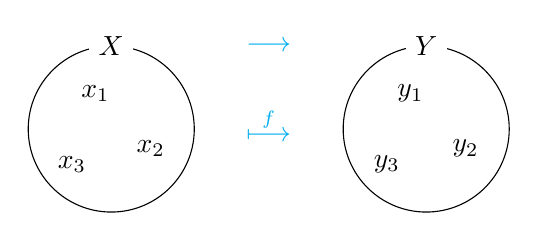
\begin{tikzpicture}[line cap=round,line join=round,>=triangle 45,x=1cm,y=1cm]
        \draw (0,3.95) circle (30pt);
        \draw (4,3.95) circle (30pt);
        \draw (-0.2,4.4) node {$x_1$};
        \draw (0.5,3.7) node {$x_2$};
        \draw (-0.5,3.5) node {$x_3$};
        \draw (3.8,4.4) node {$y_1$};
        \draw (4.5,3.7) node {$y_2$};
        \draw (3.5,3.5) node {$y_3$};
        \draw (0,5) node[fill=white] {$X$};
        \draw (4,5) node[fill=white] {$Y$};
        \draw (2,5) node[]{${\color{cyan}\longrightarrow}$};
        \draw (2,4) node[]{${\color{cyan}\stackrel{f}{\longmapsto}}$};
    \end{tikzpicture}
\end{figure}

以下,$X = \left\{x_1, x_2, x_3, \cdots, x_n\right\}$,$Y = \left\{y_1, y_2, y_3, \cdots, y_n\right\}$として,
統計処理の数式を記述する.

\subsection{Qテスト}

外れ値と疑わしいデータを棄却できるかどうかを判断する方法である.90\%の信頼限界としたQ値表が与えられている.
集合$X$の異常値を$x_a$,異常値から一番近い値を$x_{a-1}$,最大値を$x_{\mathrm{max}}$,最小値を$x_{\mathrm{min}}$とすると,以下である.

\begin{equation}
    Q = \dfrac{|x_a - x_{a-1}|}{|x_{\mathrm{max}} - x_{\mathrm{min}}|}
\end{equation}

このとき表3と比較し,$Q$の値が(2)式より大きければ異常値$x_a$を棄却できる.

\begin{table}[h]
    \centering
    \caption{各データ数$n$に対するQ値}
    \begin{tabular}{ccccccccc}
        \hline
        $n$ & 3 & 4 & 5 & 6 & 7 & 8 & 9 & 10 \\
        Q値 & 0.90 & 0.76 & 0.64 & 0.56 & 0.51 & 0.47 & 0.44 & 0.41 \\
        \hline
    \end{tabular}
\end{table}

\subsection{平均と分散}

平均は,すべてのデータを均したものである.

\begin{equation}
    平均\ \mu = \dfrac{x_1 + x_2 + x_3 + \cdots + x_i}{i}
\end{equation}

\clearpage

分散は,各データと平均との差の平均である.一般にデータの\textbf{バラつき}を表す.

\begin{equation}
    分散\ \sigma^2 = \dfrac{(x_1 - \mu)^2 + (x_2 - \mu)^2 + (x_2 - \mu)^2 + \cdots + (x_n - \mu)^2}{n}
\end{equation}

また,共分散は各成分の平均との差の積で求められる.なお$X, Y$の平均をそれぞれ$\mu_x, \mu_y$とする.
$\sum$の計算は,変数$k$が$1 \le k \le n$の範囲での\textbf{総和}であることを示している.

\begin{equation}
    共分散\ Cov(X, Y) = \dfrac{1}{n}\sum_{k=1}^{n}(x_k - \mu_x)(y_k - \mu_y)
\end{equation}

\subsection{最小二乗法}

最小二乗法は,以下の式で計算できる.

\begin{equation}
    {\color{cyan}y =} \dfrac{Cov(X, Y)}{\sigma^2_x}{\color{cyan}x} + \left(\mu_y - \dfrac{Cov(X, Y)}{\sigma^2_x}\mu_x\right)
\end{equation}

\subsection{絶対誤差と相対誤差}

絶対誤差とは,実測値と理論値の差のことである.理論値は,最小二乗法によって求めた函数に代入して求める.

\begin{equation}
    (絶対誤差) = \left|(実測値)- (理論値)\right|
\end{equation}

一方で相対誤差とは,絶対値をパーセンテージで表したものである.

\begin{equation}
    (相対誤差) = \dfrac{(絶対誤差)}{(理論値)} \times 100\ [\%]
\end{equation}

\end{document}
